\newpage
\appendix

\section{Numerical Experiments}
We now list the details related to the numerical experiments which have been left out in the main body of the paper.

\indent \quad $\bullet$ \textbf{Computational Resource.} All the numerical experiments were run in `Google Colaboratory' (``https://colab.research.google.com") and the models were in \emph{Tensorflow}.



\indent \quad $\bullet$ For experiments in \Cref{sec:exp} we used Adam [\citenum{adam}] with learning rate of $3\times 10^{-4}$, and batch size of 32.


\indent \quad $\bullet$ In \Cref{sec:exp1}, for the MNIST results in \Cref{tb:regimes}, we used the DGN architectures in \Cref{fig:dgn-prior-new} with fully connected layers instead of convolutional layers. 

\indent \quad $\bullet$ The training and test accuracy plots for the random label experiments in \Cref{sec:exp2} are shown in \Cref{fig:rand-label1,fig:rand-label2}. In particular, the fact that while training with random labels upstream the performance reaches a peak (`Best') and then it degrades (`End') can be seen in $M1(\gamma)$ in the top row of \Cref{fig:rand-label1}. 

\begin{figure}[h]
\begin{minipage}{0.99\columnwidth}
%\resizebox{\columnwidth}{!}{
\begin{tabular}{ccc}
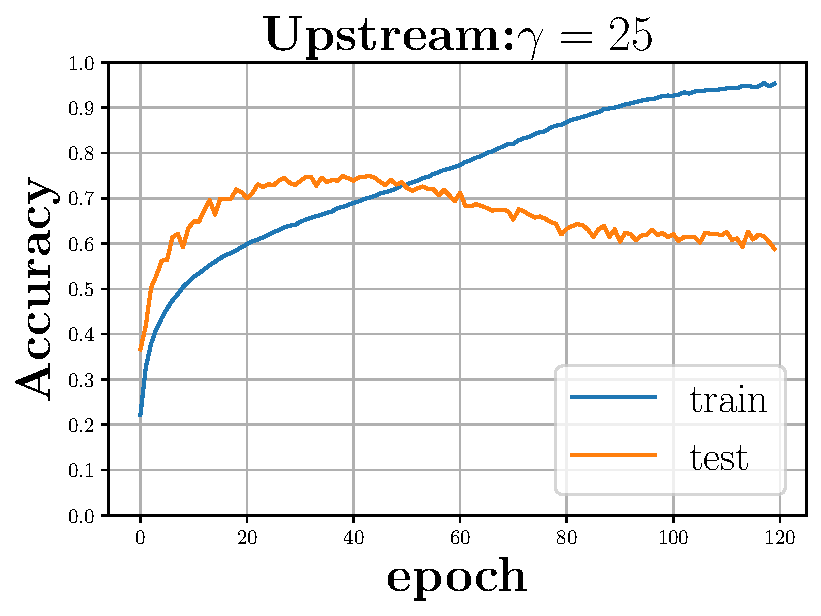
\includegraphics[scale=0.3]{figs/relu_25.pdf}&
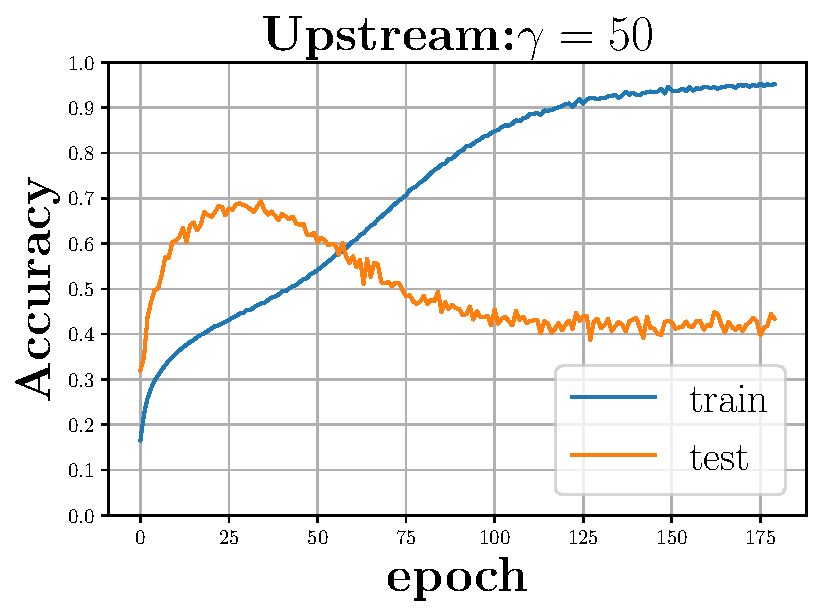
\includegraphics[scale=0.3]{figs/relu_50.pdf}&
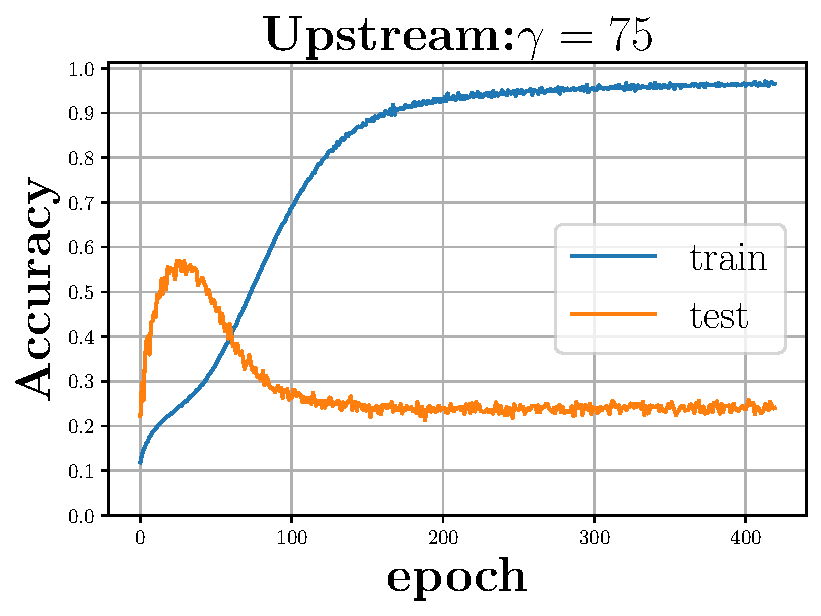
\includegraphics[scale=0.3]{figs/relu_75.pdf}
\\
 $M1(25)$ & $M1(50)$ &  $M1(75)$\\
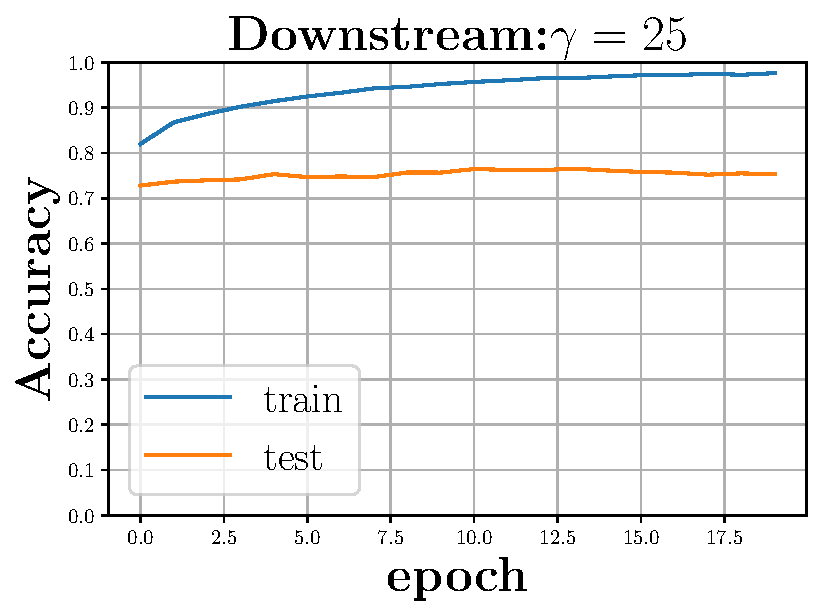
\includegraphics[scale=0.3]{figs/relu_25_good.pdf}&
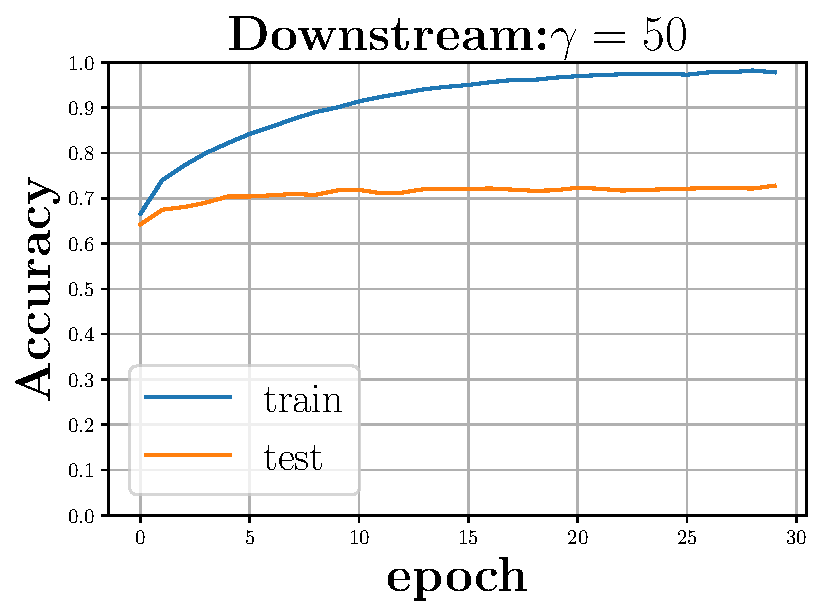
\includegraphics[scale=0.3]{figs/relu_50_good.pdf}&
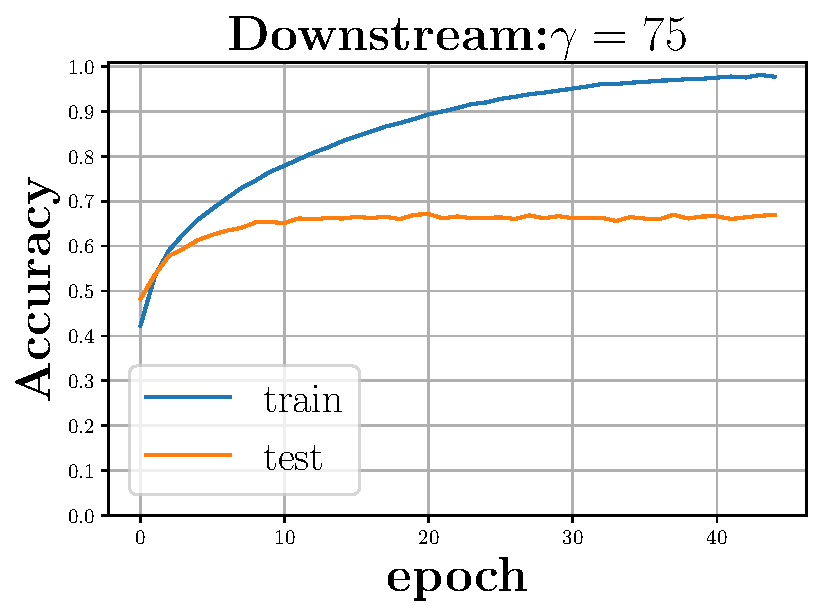
\includegraphics[scale=0.3]{figs/relu_75_good.pdf}\\
 $M4(25)$ & $M4(50)$ &  $M4(75)$
\end{tabular}
%}
\end{minipage}
\caption{Shows the upstream training with random labels $M1(\gamma)$, followed by downstream training with true labels $M4(\gamma)$. The first epochs of bottom plots is same as the last epochs in the top plots.}
\label{fig:rand-label1}

\end{figure}


\begin{figure}[h]
\begin{minipage}{0.99\columnwidth}
\resizebox{\columnwidth}{!}{
\begin{tabular}{cccccc}
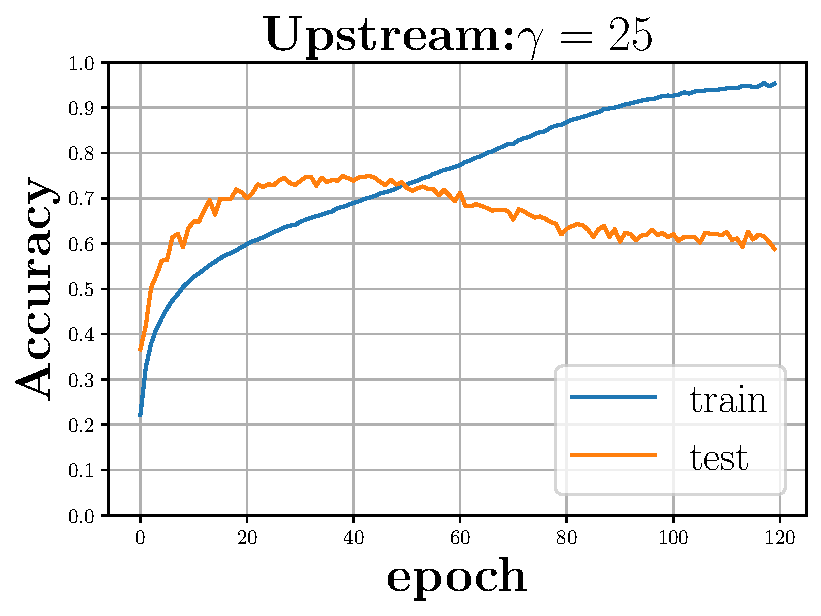
\includegraphics[scale=0.125]{figs/relu_25.pdf}&
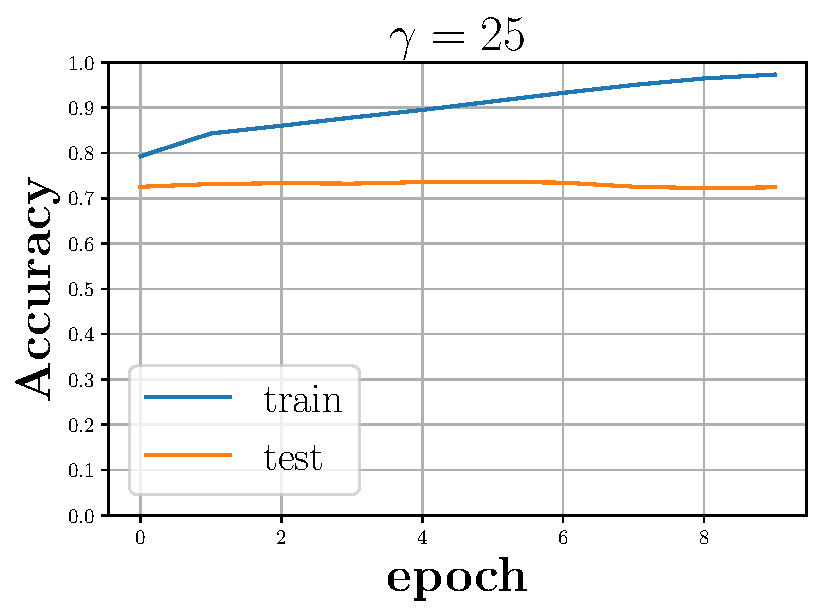
\includegraphics[scale=0.125]{figs/galu_25_good.pdf}&
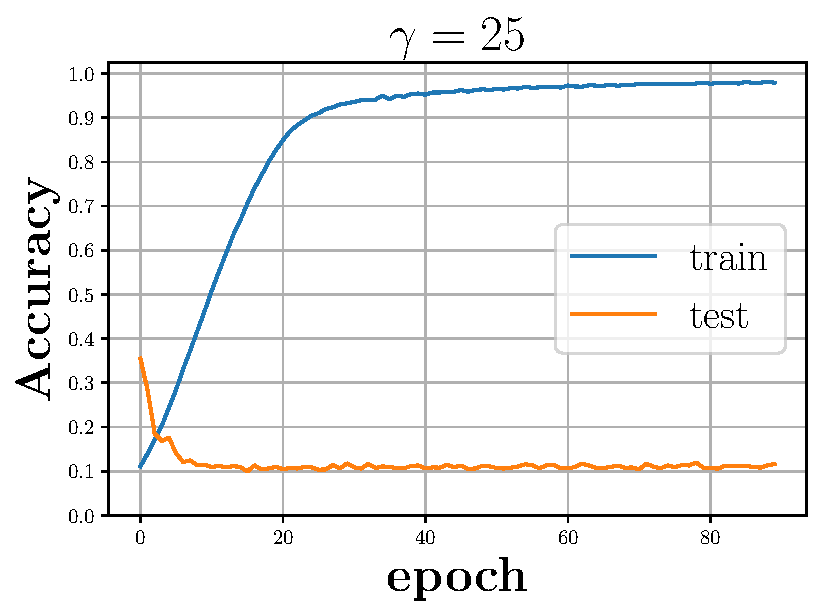
\includegraphics[scale=0.125]{figs/galu_25_bad.pdf}&
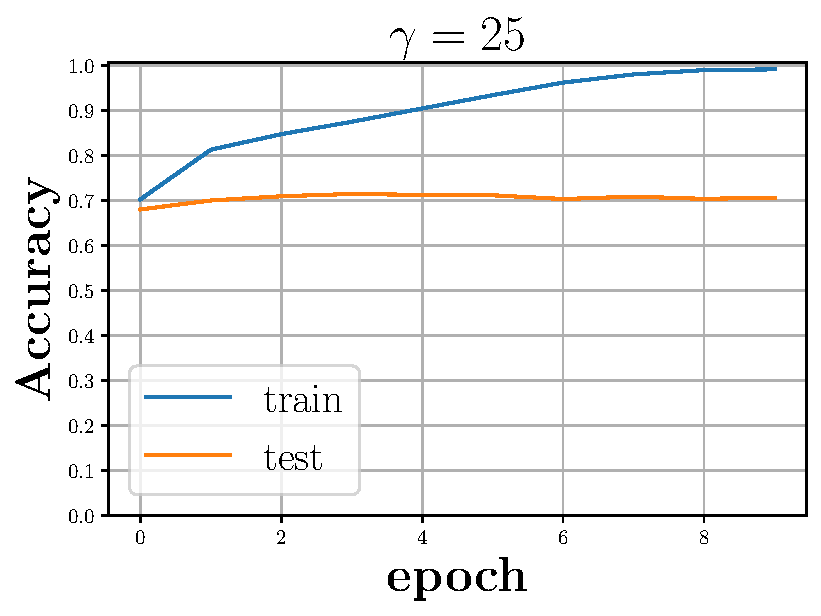
\includegraphics[scale=0.125]{figs/galu_25_bad_good.pdf}&
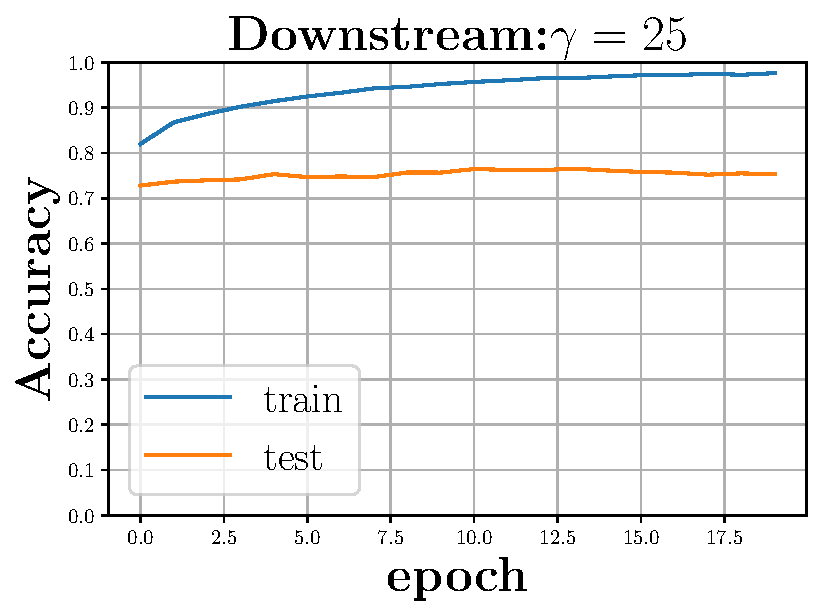
\includegraphics[scale=0.125]{figs/relu_25_good.pdf}&
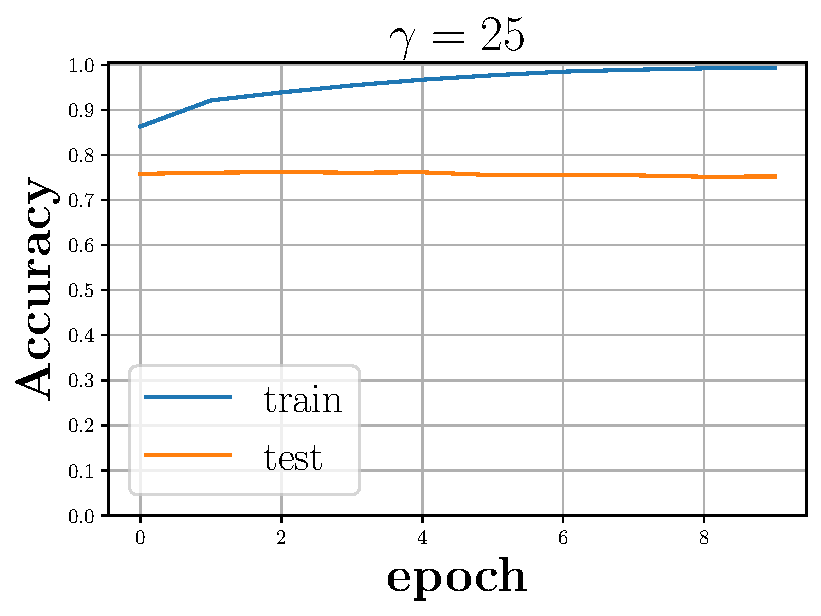
\includegraphics[scale=0.125]{figs/galu_25_recovered.pdf}
\\
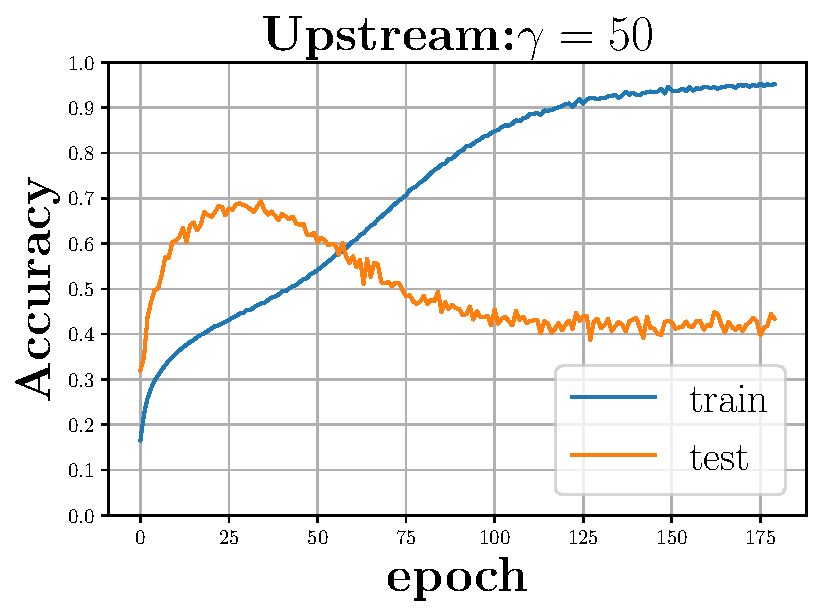
\includegraphics[scale=0.125]{figs/relu_50.pdf}&
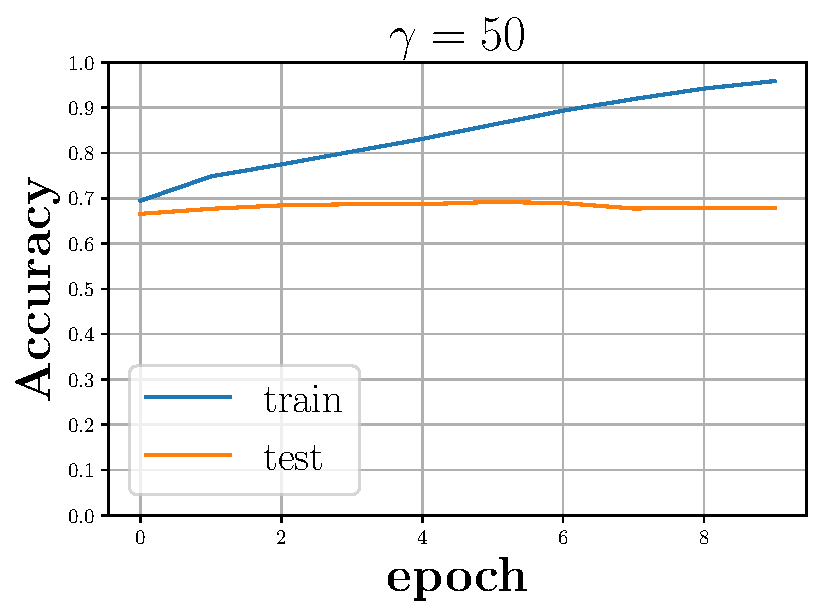
\includegraphics[scale=0.125]{figs/galu_50_good.pdf}&
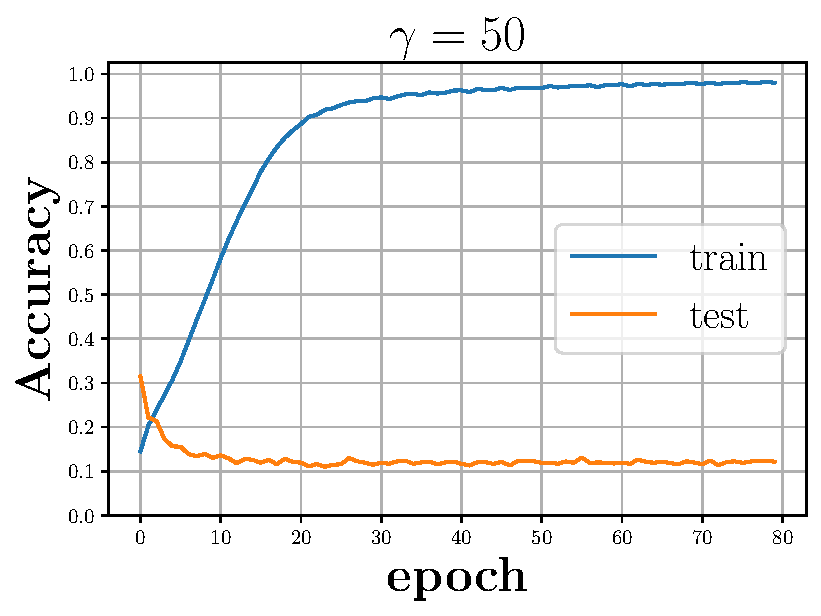
\includegraphics[scale=0.125]{figs/galu_50_bad.pdf}&
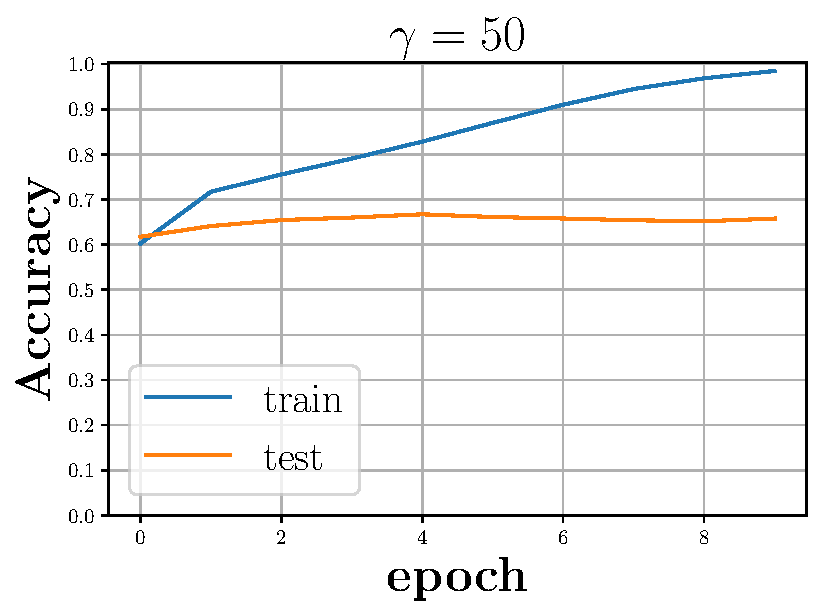
\includegraphics[scale=0.125]{figs/galu_50_bad_good.pdf}&
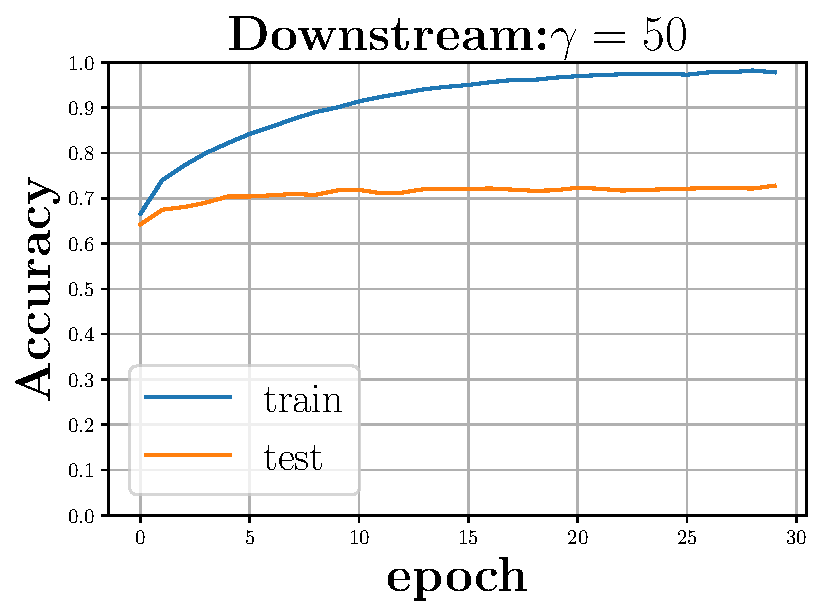
\includegraphics[scale=0.125]{figs/relu_50_good.pdf}&
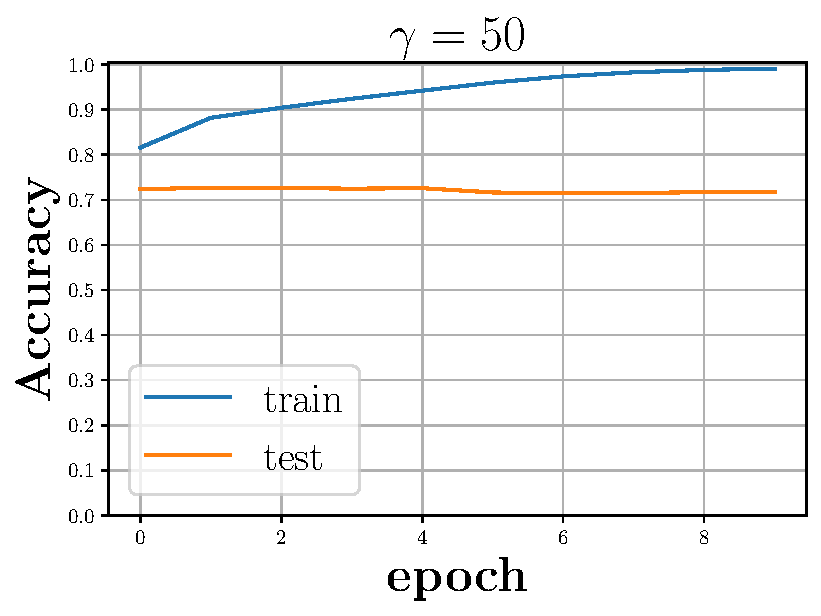
\includegraphics[scale=0.125]{figs/galu_50_recovered.pdf}
\\
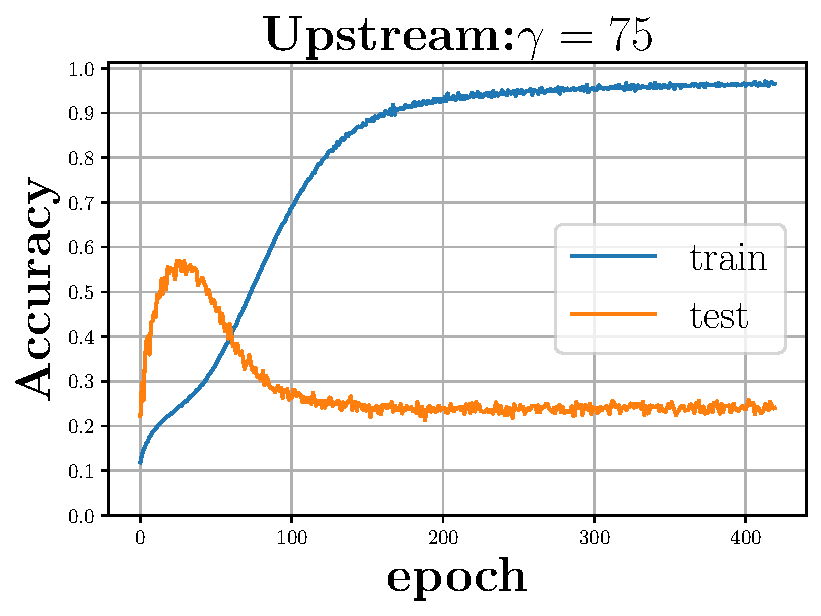
\includegraphics[scale=0.125]{figs/relu_75.pdf}&
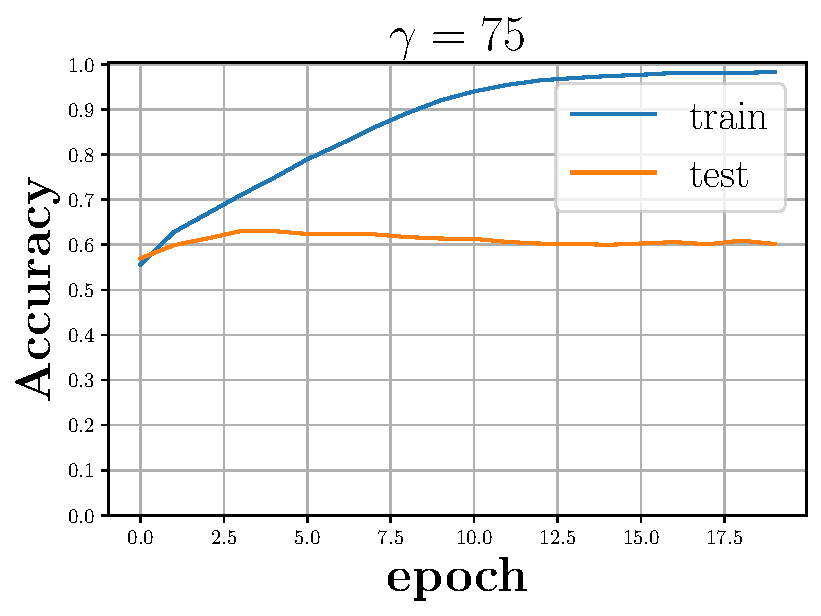
\includegraphics[scale=0.125]{figs/galu_75_good.pdf}&
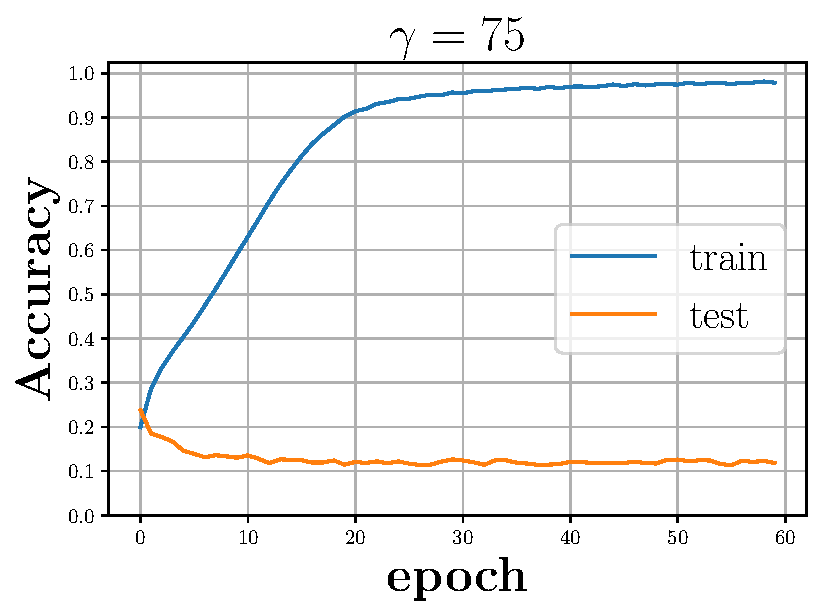
\includegraphics[scale=0.125]{figs/galu_75_bad.pdf}&
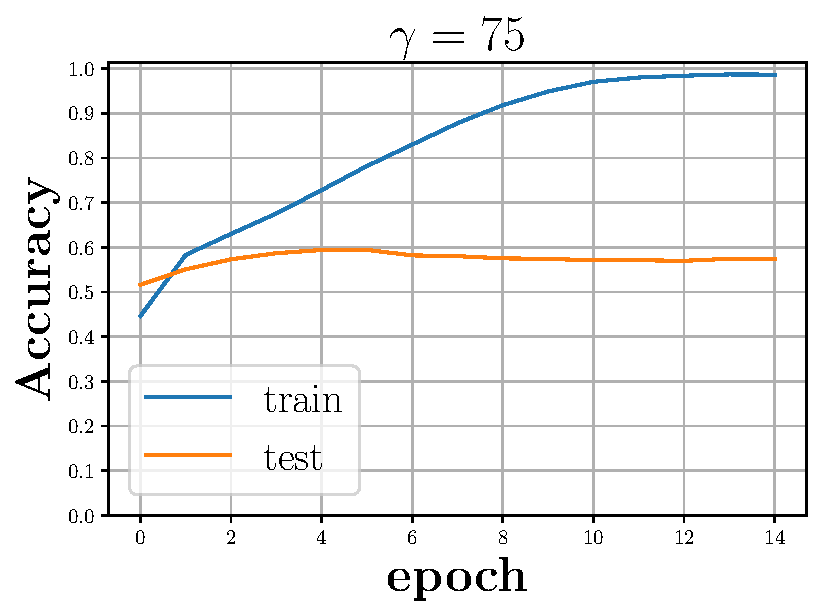
\includegraphics[scale=0.125]{figs/galu_75_bad_good.pdf}&
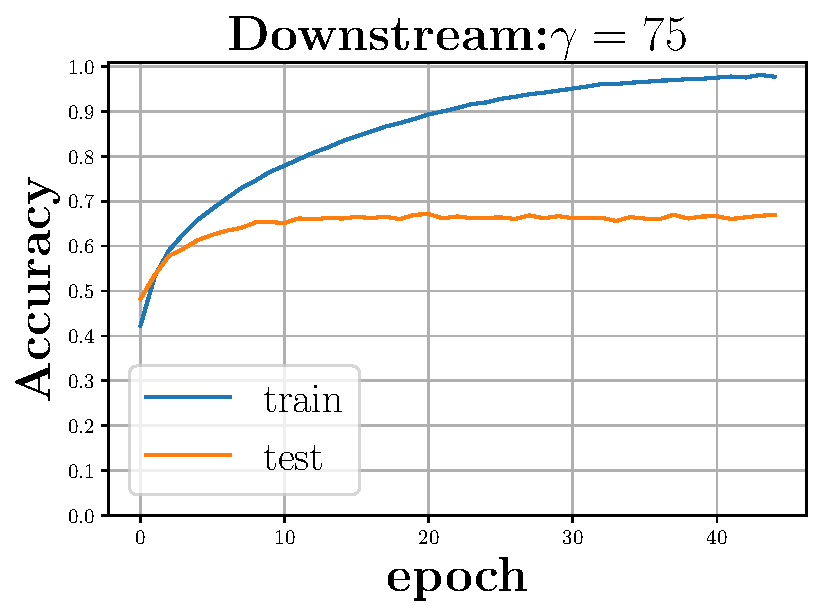
\includegraphics[scale=0.125]{figs/relu_75_good.pdf}&
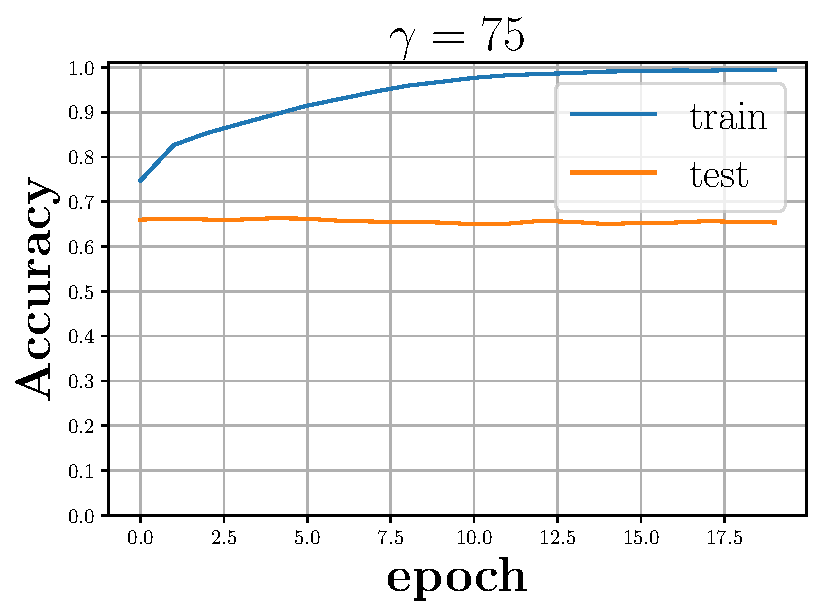
\includegraphics[scale=0.125]{figs/galu_75_recovered.pdf}\\
\tiny{M1}&\tiny{M2}&\tiny{M3:US}&\tiny{M3:DS}&\tiny{M4}&\tiny{M5}\\
\end{tabular}
}
\end{minipage}
\caption{Shows the training and test accuracy plots of a single run for models $M1,M2,M3,M4$ and $M5$.}
\label{fig:rand-label2}
\end{figure}

\indent \quad $\bullet$ In \Cref{sec:interpret}, the code for VGG19 architecture is from the repository ``https://github.com/gahaalt/resnets-in-tensorflow2", and the ResNet architecture called \texttt{DavidNet} is from the repository ``https://github.com/davidcpage/cifar10-fast". The \texttt{DGN-No-Act}s based on these architectures were derived in a manner described in \Cref{sec:interpret}.

\indent \quad $\bullet$ For VGG19 (and the corresponding \texttt{DGN-No-Act}), we used \emph{SGD} optimiser with momentum $0.9$ and the following learning rate schedule (as suggested in ``https://github.com/gahaalt/resnets-in-tensorflow2") : for iterations $[0, 400)$ learning rate was $0.01$,  for iterations $[400, 32000)$ the learning rate was $ 0.1$, for iterations $[32000, 48000)$ the learning rate was $0.01$, for iterations $[48000, 64000)$ the learning rate was $0.001$. The batch size was $128$. The models were trained till $32$ epochs.


\indent \quad $\bullet$ For \texttt{DavidNet} (and the corresponding \texttt{DGN-No-Act}), we used \emph{SGD} optimiser with momentum $0.9$, learning rate $0.4$, batch size of $512$, weight decay of $5\times 10^{-4}$ (as suggested in ``https://github.com/davidcpage/cifar10-fast").





\section{Fully Connected}
Here, we present the formal definition for the neural path features and neural path values for the fully connected case in \Cref{def:formal-npf-npv}.  The layer-by-layer way of expressing the computation in a DNN of width `$w$' and depth `$d$' is given below.
\begin{table}[h]
\centering
\begin{tabular}{| ll lll|}\hline
 Input Layer &:& $z_{x,\Theta}(\cdot,0)$ &$=$ &$x$ \\
Pre-Activation&:& $q_{x,\Theta}(\iout,l)$& $=$ & $\sum_{\iin}\Theta(\iin,\iout,l) \cdot z_{x,\Theta}(\iin,l-1) $\\
Gating&:& $G_{x,\Theta}(\iout,l)$& $=$ & $\mathbf{1}_{\{q_{x,\Theta}(\iout,l)>0\}}$\\
Hidden Layer Output &:&$z_{x,\Theta}(\iout,l)$ & $=$ & $q_{x,\Theta}(\iout,l)\cdot G_{x,\Theta}(\iout,l)$\\
Final Output &:&$\hat{y}_{\Theta}(x)$ & $=$ & $\sum_{\iin}\Theta(\iin,\iout, d)\cdot z_{x,\Theta}(\iin,d-1)$\\\hline
\end{tabular}
\caption{\small{Information flow in a FC-DNN with ReLU. Here, `$q$'s are pre-activation inputs, `$z$'s are output of the hidden layers, `$G$'s are the gating values. $l\in[d-1]$ is the index of the layer, $\iout$ and $\iin$ are indices of  nodes in the current and previous layer respectively.}}
\label{tb:basic}
\end{table}

\begin{notation}
Index maps identify the nodes through which a path $p$ passes. The ranges of index maps $\Ifeat_l$, $\I_l,l\in[d-1]$ are $[\din]$ and $[w]$ respectively.  $\I_d(p)=1,\forall p\in[\Pfc]$.
\end{notation}

\begin{definition}\label{def:formal-npf-npv} Let $x\in\R^{\din}$ be the input to the DNN. For this input, 

(i)  $A_{\Theta}(x,p)\eqdef\Pi_{l=1}^{d-1} G_{x,\Theta}(\I_l(p),l)$ is the activity of a path.

(ii)  $\phi_{x,\Theta}\eqdef \left( x(\Ifeat_0(p))A_{\Theta}(x,p), p\in[\Pfc]\right)\in\R^{\Pfc}$ is the {neural path feature} (NPF).

(iii)  $v_{\Theta}\eqdef \left( \Pi_{l=1}^d \Theta(\I_{l-1}(p),\I_l(p),l), p\in[\Pfc]\right)\in\R^{\Pfc}$ is the {neural path value} (NPV).
\end{definition}

We now restate \Cref{th:main} in the notation introduced in \Cref{tb:basic}.
\begin{theorem}[Product of Kernels Theorem] Under \Cref{assmp:main}  ($\sigma=\frac{\cscale}{\sqrt{w}}$) for FC-DGN : 
\begin{align*}
\kv_{\Tdgn_0}(x,x') &\stackrel{(a)}{\ra} d\cdot \sigma^{2(d-1)} \cdot H_{\Tf_0}(x,x'), \quad\text{as}\,\, w\ra\infty \\
&\stackrel{(b)}{=} d\cdot \cscale^{2(d-1)} \cdot \left(\ip{ x,x'} \cdot \Pi_{l=1}^{d-1} \frac{\ip{G_{x,\Theta}(\cdot,l), G_{x',\Theta}(\cdot,l)}}w\right)
\end{align*}
\end{theorem} 

\begin{proof}
Here $(a)$ is same as Theorem~5.1 in [\citenum{npk}]. From \Cref{lm:npk}, we know that $H_{\Theta}(x,x')=\ip{x,x'}_{\Lambda_{\Theta}(\cdot,x,x')}$, and that in the case of fully connected networks $\Lambda_{\Theta}(i,x,x')$ does not change with $i$. $(b)$ follows from the fact the total number of paths simultaneously `active' is equal to the product of the total number of gates simultaneously active in each layer, i.e., $\Lambda_{\Theta}(x,x')=\ip{G_{x,\Theta}(\cdot,l), G_{x',\Theta}(\cdot,l)}$. 
\end{proof}

\section{Convolution with pooling}
In this section, we define NPFs and NPV in the presence of convolution with pooling. This requires three key steps (i) treating pooling layers like gates/masks (see \Cref{def:pooling}) (ii) bundling together the paths that share the same path value
(due to weight sharing in convolutions, see \Cref{def:bundle}),  and (iii) re-defining the NPF and NPV for bundles (see \Cref{def:convnps}). Weight sharing due to convolutions and pooling makes the NPK rotationally invariant \Cref{lm:cnnnpk}. We begin by describing the architecture.

\textbf{Architecture:} We consider (for sake of brevity) a $1$-dimensional\footnote{The results follow in a direct manner to any form of circular convolutions.} convolutional neural network with circular convolutions, with $\dc$ convolutional layers ($l=1,\ldots,\dc$), followed by a \emph{global-average/max-pooling} layer ($l=\dc+1$) and $\dfc$ ($l=\dc+2,\ldots,\dc+\dfc+1$) FC  layers. The convolutional window size is $\wconv<\din$, the number of filters per convolutional layer as well as the width of the FC is $w$. 

\textbf{Indexing:} Here $\iin/\iout$ are the indices (taking values in $[w]$) of the input/output filters. $\icin$ denotes the indices of the convolutional window taking values in $[\wconv]$. $\ifout$ denotes the indices (taking values in $[\din]$, the dimension of input features) of individual nodes in a given output filter. The weights of layers $l\in[\dc]$ are denoted by $\Theta(\icin,\iin,\iout,l)$ and for layers $l\in[\dfc]+\dc$ are denoted by $\Theta(\iin,\iout,l)$. The pre-activations, gating and hidden unit outputs are denoted by $q_{x,\Theta}(\ifout,\iout,l)$,  $G_{x,\Theta}(\ifout,\iout,l)$, and $z_{x,\Theta}(\ifout,\iout,l)$ for layers $l=1,\ldots, \dc$.


\begin{definition}[Circular Convolution]
For $x\in\R^{\din}$, $i\in[\din]$ and $r\in\{0,\ldots,\din-1\}$, define :

(i) $i\oplus r = i+r$, for $i+r \leq \din$ and $i\oplus r =i+r-\din$, for $i+r>\din$.

(ii) $rot(x,r)(i)=x(i\oplus r), i\in[\din]$.

(iii) $q_{x,\Theta}(\ifout,\iout,l)=\sum_{\icin,\iin}\Theta(\icin,\iin,\iout,l)\cdot z_{x,\Theta}(\ifout\oplus (\icin-1),\iin,l-1)$. 
\end{definition}
\begin{definition}[Pooling]\label{def:pooling}
Let $G^{\text{pool}}_{x,\Theta}(\ifout,\iout,\dc+1)$ denote the pooling mask, then we have
\centerline{
$z_{x,\Theta}(\iout, \dc+1) =\sum_{\ifout} z_{x,\Theta}(\ifout,\iout,\dc)\cdot G^{\text{pool}}_{x,\Theta}(\ifout,\iout,\dc+1),$
}
where in the case of \emph{global-average-pooling} $G^{\text{pool}}_{x,\Theta}(\ifout,\iout,\dc+1)=\frac{1}{\din},\forall \iout\in[w], \ifout\in[\din]$, and in the case of \emph{$\max$-pooling},  
for a given $\iout\in[w]$, $G^{\text{pool}}_{x,\Theta}(i_{\max},\iout,\dc+1)=1$ where $i_{\max}=\arg\max_{\ifout}z_{x,\Theta}(\ifout,\iout,\dc)$, and $G^{\text{pool}}_{x,\Theta}(\ifout,\iout,\dc+1)=0,\forall \ifout\neq i_{\max}$.
\end{definition}

\begin{table}[t]
\centering
\begin{tabular}{|c l lll|}\hline
IL&: &$z_{x,\Theta}(\cdot,1,0)$ &$=$ &$x$ \\\hline\hline
\multicolumn{5}{|l|}{Convolutional Layers, $l\in[\dc]$}\\\hline\hline
PA&: & $q_{x,\Theta}(\ifout,\iout,l)$& $=$ & $\sum_{\icin,\iin}\Theta(\icin,\iin,\iout,l)\cdot z_{x,\Theta}(\ifout\oplus (\icin-1),\iin,l-1)$\\
GV&: &$G_{x,\Theta}(\ifout,\iout,l)$& $=$ & $\mathbf{1}_{\{q_{x,\Theta}(\ifout,\iout,l)>0\}}$\\
HUO&: &$z_{x,\Theta}(\ifout,\iout,l)$ & $=$ & $q_{x,\Theta}(\ifout,\iout,l)\cdot G_{x,\Theta}(\ifout,\iout,l)$\\\hline\hline
\multicolumn{5}{|l|}{GAP Layers, $l=\dc+1$}\\\hline\hline
%HUO&: &${z}_{x,\Theta}(\iout,l)$ & $=$ & $\frac{1}{\din}\sum_{i\in [\din]} z_{x,\Theta}(i,\iout,l-1)$\\\hline\hline
HUO&: &$z_{x,\Theta}(\iout, \dc+1)$ & $=$ &$\sum_{\ifout} z_{x,\Theta}(\ifout,\iout,\dc)\cdot G^{\text{pool}}_{x,\Theta}(\ifout,\iout,\dc+1)$\\\hline\hline
\multicolumn{5}{|l|}{Fully Connected Layers, $l\in[\dfc]+(\dc+1)$}\\\hline\hline
PA&: & $q_{x,\Theta}(\iout,l)$& $=$ & $\sum_{\iin}\Theta(\iin,\iout,l) \cdot z_{x,\Theta}(\iin,l-1) $\\
GV&: &$G_{x,\Theta}(\iout,l)$& $=$ & $\mathbf{1}_{\{(q_{x,\Theta}(\iout,l))>0\}}$\\
HUO&: &$z_{x,\Theta}(\iout,l)$ & $=$ & $q_{x,\Theta}(\iout,l)\cdot G_{x,\Theta}(\iout,l)$\\
FO&: & $\hat{y}_{\Theta}(x)$ & $=$ & $\sum_{\iin}\Theta(\iin,\iout, d)\cdot z_{x,\Theta}(\iin,d-1)$\\\hline
\end{tabular}
\caption{Here IL, PA, GV, HUO, GL and FO are abbreviations for input layer, pre-activation, gating values, hidden unit output, GAP-layer and final output respectively.}
\label{tb:cconv}
\end{table}

\begin{proposition}
The total number of paths in a CNN is given by  $\Pcnn=\din(\wconv w)^{\dc}w^{(\dfc-1)}$.
\end{proposition}

\begin{notation}[Index Maps]
The ranges of index maps $\Ifeat_l$,  $\Iconv_l$, $\I_l$ are $[\din]$, $[\wconv]$ and $[w]$ respectively. 
\end{notation}

\begin{definition}[Bundle Paths of Sharing Weights]\label{def:bundle}
Let $\hat{P}^{\text{cnn}}=\frac{\Pcnn}{\din}$, and $\{B_1,\ldots, B_{\hat{P}^{\text{cnn}}}\}$ be a collection of sets such that $\forall i,j\in [\hat{P}^{\text{cnn}}], i\neq j$ we have $B_i\cap B_j=\emptyset$ and $\cup_{i=1}^{\hat{P}^{\text{cnn}}}B_i =[\Pcnn]$. Further,  if paths $p,p' \in B_i$, then $\Iconv_l(p)=\Iconv_l(p'), \forall l=1,\ldots, \dc$ and $\I_l(p)=\I_l(p'), \forall l=0,\ldots, \dc$.
\end{definition}

\begin{proposition}\label{prop:bundle}
There are exactly $\din$ paths in a bundle.
\end{proposition}

\begin{definition}\label{def:convnps} Let $x\in\R^{\din}$ be the input to the CNN. For this input, 
\begin{tabular}{rlp{12cm}}
$A_{\Theta}(x,p)$&$\eqdef$&$\left(\Pi_{l=1}^{\dc+1} G_{x,\Theta}(\Ifeat_l(p),\I_l(p),l)\right)\cdot\left(\Pi_{l=\dc+2}^{\dc+\dfc+1} G_{x,\Theta}(\I_l(p),l)\right)$\\
$\phi_{x,\Theta}(\hat{p})$&$\eqdef$&$ \sum_{\hat{p}\in B_{\hat{p}}}x(\Ifeat_0(p))A_{\Theta}(x,p)$\\
$v_{\Theta}(B_{\hat{p}})$&$\eqdef$&$ \left(\Pi_{l=1}^{\dc} \Theta(\Iconv_{l}(p),\I_{l-1}(p),\I_{l}(p),l)\right) \cdot\left( \Pi_{l=\dc+2}^{\dc+\dfc+1} \Theta(\I_{l-1}(p),\I_l(p),l)\right)$ 
\end{tabular}
\begin{center}
\begin{tabular}{|c|c|}\hline
NPF &$\phi_{x,\Theta}\eqdef (\phi_{x,\Theta}(B_{\hat{p}}),\hat{p}\in [\hat{P}^{\text{cnn}}])\in\R^{\hat{P}^{\text{cnn}}}$\\\hline
NPV& $v_{\Theta}\eqdef (v_{\Theta}(B_{\hat{p}}),\hat{p}\in [\hat{P}^{\text{cnn}}])\in\R^{\hat{P}^{\text{cnn}}}$\\\hline
\end{tabular}
\end{center}
\end{definition}



\begin{lemma}[Rotational Invariant Kernel]\label{lm:cnnnpk}
Let $H^{\text{cnn}}_{\Theta}$ denote the NPK of a CNN, then 
\begin{align*}
H^{\text{cnn}}_{\Theta}(x,x')&=\sum_{r=0}^{\din-1} \ip{x,rot(x',r)}_{\Lambda(\cdot, x,rot(x',r))}\\&=\sum_{r=0}^{\din-1} \ip{rot(x,r),x'}_{\Lambda(\cdot, rot(x,r),x')}
\end{align*}
\end{lemma}

\begin{proof}
For the CNN architecture considered in this paper, each bundle has exactly $\din$ number of paths, each one corresponding to a distinct input node. For a bundle $b_{\hat{p}}$, let $b_{\hat{p}}(i),i\in[\din]$ denote the path starting from input node $i$.
\begin{align*}
&\sum_{\hat{p}\in [\hat{P}]} \Bigg(\sum_{i,i'\in[\din]} x(i) x'(i') A_{\Theta}\left(x,b_{\hat{p}}(i)\right) A_{\Theta}\left(x',b_{\hat{p}}(i')\right) \Bigg)\\
=&\sum_{\hat{p}\in [\hat{P}]}\Bigg(\sum_{i\in[\din],i'=i\oplus r, r\in\{0,\ldots,\din-1\}} x(i) x'(i\oplus r) A_{\Theta}\left(x,b_{\hat{p}}(i)\right) A_{\Theta}\left(x',b_{\hat{p}}(i\oplus r)\right)\Bigg)\\
=&\sum_{\hat{p}\in [\hat{P}]}\Bigg(\sum_{i\in[\din], r\in\{0,\ldots,\din-1\}} x(i) rot(x',r)(i) A_{\Theta}\left(x,b_{\hat{p}}(i)\right) A_{\Theta}\left(rot(x',r),b_{\hat{p}}(i)\right)\Bigg)\\
=&\sum_{r=0}^{\din-1} \Bigg(\sum_{i\in[\din]} x(i) rot(x',r)(i) \sum_{\hat{p}\in [\hat{P}]}  A_{\Theta}\left(x,b_{\hat{p}}(i)\right) A_{\Theta}\left(rot(x',r),b_{\hat{p}}(i)\right)\Bigg)\\
=&\sum_{r=0}^{\din-1}\Bigg(\sum_{i\in[\din]} x(i) rot(x',r)(i) \Lambda_{\Theta}(i,x,rot(x',r))\Bigg)\\
=&\sum_{r=0}^{\din-1} \ip{x,rot(x',r)}_{\Lambda_{\Theta}(\cdot,x,rot(x',r))}
\end{align*}
\end{proof}


In what follows we re-state \Cref{th:mainconv}.

\begin{theorem} Let $\sigcnn=\frac{\cscale}{\sqrt{w\wconv}}$ for the convolutional layers and $\sigfc=\frac{\cscale}{\sqrt{w}}$ for FC layers. Under \Cref{assmp:main}, as $w\ra\infty$, with  $\bcnn = \ \left(\dconv \sigcnn^{2(\dconv-1)}\sigfc^{2\dfc}+\dfc \sigcnn^{2\dconv}\sigfc^{2(\dfc-1)}\right)$ we have:
\begin{align*}
&\kv_{\Tdgn_0}\ra\quad \frac{\bcnn}{{\din}^2} \cdot H^{\text{cnn}}_{\Tf_0},\,\,\text{(for global-average-pooling)}\\
&\kv_{\Tdgn_0}\ra \quad{\bcnn} \cdot H^{\text{cnn}}_{\Tf_0},\,\,\text{(for global-max-pooling)}\\
\end{align*}
\end{theorem}

\begin{proof}
Follows from Theorem~5.1 in [\citenum{npk}].
\end{proof}

\section{Residual Networks with Skip connections}

As a consequence of the skip connections, within the ResNet architecture there are $2^b$ sub-FC networks (see \Cref{def:subfcdnn}). The total number of paths $\Pres$ in the ResNet is equal to the summation of the paths in these $2^b$ sub-FC networks (see \Cref{prop:resnetpath}). Now, The neural path features and the neural path value are $\Pres$ dimensional quantities, obtained as the concatenation of the NPFs and NPV of the $2^b$ sub-FC networks. 

\begin{proposition}\label{prop:resnetpath}
The total number of paths in the ResNet is  $\Pres = \din \cdot\sum_{i=0}^b \binom{b}{i} w^{(i+2)\dblock-1}$.
\end{proposition}

\begin{lemma}[Sum of Product Kernel]\label{lm:sumofproduct}
Let $H^{\text{res}}_{\Theta}$ be the NPK of the ResNet, and $H^{\J}_{\Theta}$ be the NPK of the sub-FC-DNN within the ResNet obtained by ignoring those skip connections in the set $\J$. Then, \begin{align*}H^{\text{res}}_{\Theta}=\sum_{\J\in 2^{[b]}}H^{\J}_{\Theta}\end{align*}
%\begin{align*}
%\end{align*}
\end{lemma}
\begin{proof}
Proof is complete by noting that the NPF of the ResNet is a concatenation of the NPFs of the $2^b$ distinct sub-FC-DNNs within the ResNet architecture.
\end{proof}

We re-state \Cref{th:mainres}
\begin{theorem} Let $\sigma=\frac{\cscale}{\sqrt{w}}$. Under \Cref{assmp:main}, as $w\ra\infty$,  for $\bres^{\J} = (|\J| +2)\cdot\dblock\cdot \sigma^{2\big( (|\J|+2)\dblock-1\big)}$,
\begin{align*}
\kv_{\Tdgn_0}\ra \sum_{\J\in 2^{[b]}}  \bres^{\J} H^{\J}_{\Tf_0}
\end{align*}
\end{theorem}


\begin{proof}
Follows from Theorem~5.1 in [\citenum{npk}].
\end{proof}


